Dans ce problème, on se propose d’étudier l’évolution de la concentration dans le sang d’un médicament ingéré par une personne pour la première fois.

\medskip

{\bf Partie A}\par \medskip

Soit $t$ le temps (exprimé en heures) écoulé depuis l’ingestion de ce produit. Cette concentration, en gramme par litre de sang, est une fonction $f$ de la variable $t$ définie sur l’intervalle $[0~;~+\infty[$ qui est solution de l’équation différentielle :

$$(E) : \quad y'(t)+y(t)= a\e^{-t} $$

Avec $a$ est une constante positive dépendant de la personne et de la quantité de médicament absorbée, et avec la condition initiale : $f (0) = 0$.

On suppose ici que $a = 5$, l’équation (E) s’écrit alors : $y'(t)+y(t)= 5\e^{-t}$

\begin{enumerate}
	\item Donner, puis résoudre l'équation homogène (E$_0$) :\par \vspace*{0.5cm}

	\Lignes{2}
	\item A l’aide du logiciel Géogébra, déterminer le nombre réel $m$ pour que la fonction $p$ définie sur $[0~;~+\infty[$ par : $p(t) = m~t~\e^{-t}$ soit une solution particulière de l'équation différentielle (E), et donner l’expression de $p$. 
	
	%{\it On prendra des curseurs allant de $0$ à $40$ par pas de $2$}\\
	
	On trouve : \hfill $m=$\makebox[0.1\linewidth]{\dotfill} \hfill $p(x)=$\makebox[0.3\linewidth]{\dotfill}

	\smallskip
	
	\appelprof
	
	\item En déduire l'ensemble des solutions de (E) : \par \vspace*{0.5cm}

	\Lignes{1}
	\item Déterminer, par un calcul, la solution $f$ de (E) répondant aux contraintes de l'énoncé : \par \vspace*{0.5cm}

	\Lignes{3}

\end{enumerate}

{\bf Partie B}\par \medskip

On considère la fonction $f$ définie sur $[0~;~+\infty[$ par : $f(t)=5~t~\e^{-t}$

\begin{enumerate}
	\setcounter{enumi}{4}
	\item À l'aide de l'outil calcul formel de Géogebra, étudier les varations de $f$ sur $[0~;~+\infty[$ :
	
	\begin{enumerate}
		\item Déterminer $f'(t)$.~ \dotfill \medskip
		
		\item Résoudre sur $\left[0~;~+\infty\right[$ : $f'(t)=0$ \hspace*{0.5cm} \dotfill \par \medskip
		
		\item \hspace*{4.2cm}$f'(t)\geq 0$ \hspace*{0.5cm} \dotfill \par \medskip
		
		\item Compléter alors le tableau de variation complet de la fonction $f$ sur $\left[0~;~+\infty\right[$ :
		
		{\it \small On fera figurer les valeurs au bout des flèches}
		
		\begin{center}
		\begin{tikzpicture}
	   \tkzTabInit[lgt=3]{$t$ / 1 , signe de $f'(t)$ / 1, variations de $t$ / 2}{$ $, $ $, $ $, $ $}
		\end{tikzpicture}	
		\end{center}
		\end{enumerate}	
	
	\item On a $\ds{\lim_{t\rightarrow+\infty}f(t)=0}$. Comment interpréter médicalement ce résultat ?\par \vspace*{0.5cm}

	\Lignes{1}
	\item Pour une concentration supérieur à 1 gramme par litre de sang, il y a risque de somnolence.
	
	Déterminer, à l’aide de la courbe de f, combien de temps après la prise du médicament le risque de somnolence n’est plus. Donner le résultat en heures et minutes.\par \vspace*{0.5cm}

	\Lignes{3}
\end{enumerate}

{\bf Partie C}

\begin{enumerate}
	\setcounter{enumi}{7}
	\item Soit $F$ la fonction définie sur $\left[0~;~+\infty\right[$ par : $F(t)=(-5~t-5)\e^{-t}$
	\begin{enumerate}
		\item Vérifier, par un calcul, que $F$ est une primitive de $f$. \par \vspace*{0.5cm}

	\Lignes{4}
		
		\item La concentration moyenne du médicament (en gramme par litre de sang) durant la première heure est donnée par : $\ds{T_m = \int_0^1f(t)\text{d}t}$
		
		Rappler la formule permettant de calculer $T_m$ à l'aide de $F$, puis donner une valeur approchée à $0,01$ près.\par \vspace*{0.5cm}

	\Lignes{2}
	\end{enumerate}
\end{enumerate}